\section{Videooptagelser}
\label{VideooptagelserValgAfGestikker}
%
I følgende afsnit vil det blive beskrevet og vist, hvordan videoer af henholdsvis gestikker for pause og start, skift musiknummer og ændring af volumen er udarbejdet. Videoerne, der viser bevægelserne i hver gestik, er vedlagt i det \textbf{elektroniske bilag}.

Til test af hvilke gestikker der fungerer til de forskellige funktioner i et musikanlæg, er det relevant at kunne vise de forskellige gestikker, for at testpersonerne på den måde ikke er i tvivl om hvilke gestikker der menes. Til udarbejdelsen af videoerne bruges et Canon Powershot s110 kamera på stativ, der både optager billede og lyd. Videoerne er optaget med en 45$^{\circ}$'s vinkel, et halvnært perspektiv samt en neutral baggrund og et neutralt ansigtsudtryk, hvilket er illustreret på \autoref[fig:Tryk]. På denne måde kan gestikken ses tydelig, både med dybde og størrelse, uden at der er forstyrrelser i form af øjenkontakt med demonstratoren eller sjove grimasser. Under optagelserne sættes der musik på, som styres fra en computer. Til at pause og starte musikken bruges musiknummeret \enquote{Stay} fra Zedd og Alessia Cara (2017). Til at skifte musiknumer bruges musiknumrene \enquote{Closer} fra The Chainsmokers ft. Halsey (2016) og \enquote{Galway Girl} fra Ed Sheeran (2017) og til at ændre volumen bruges musiknummeret \enquote{You Don't Know Me} fra Jax Jones ft. RAYE (2017). Når en gestik for eksempelvis pause laves, pauses musikken fra computeren og videoen demonstrerer på den måde, hvordan musik kan pauses ved udførelse af en gestik. De resterende funktioner optages på tilsvarende måde.

%
%\begin{figure}[H]
%	\centering
%	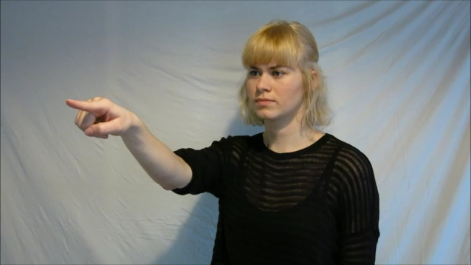
\includegraphics[resolution=300,width=0.70\textwidth, angle=-90]{Tryk}
%	\caption{Snapshot fra pause og start videoen.}
%	\label{fig:Tryk}
%\end{figure}
%\noindent
%

Optagelsen af videoerne er redigeret i Windows Movie Maker version 2012. Her er de forskellige gestik-par blevet adskilt, hvorefter det er tydeliggjort hvornår hver ny gestik starter. Efter alle gestikker er demonstreret på videoen vises et oversigts-billede, hvor alle gestikkerne kan ses med nummerering og pile, der viser gestikkens retning. Disse tre oversigts-billeder er illustreret på \autoref{fig:OversigtPauseStart}, \autoref{fig:OversigtSkift} og \autoref{fig:OversigtVolumen}.

%
%\begin{figure}[H]
%	\centering
%	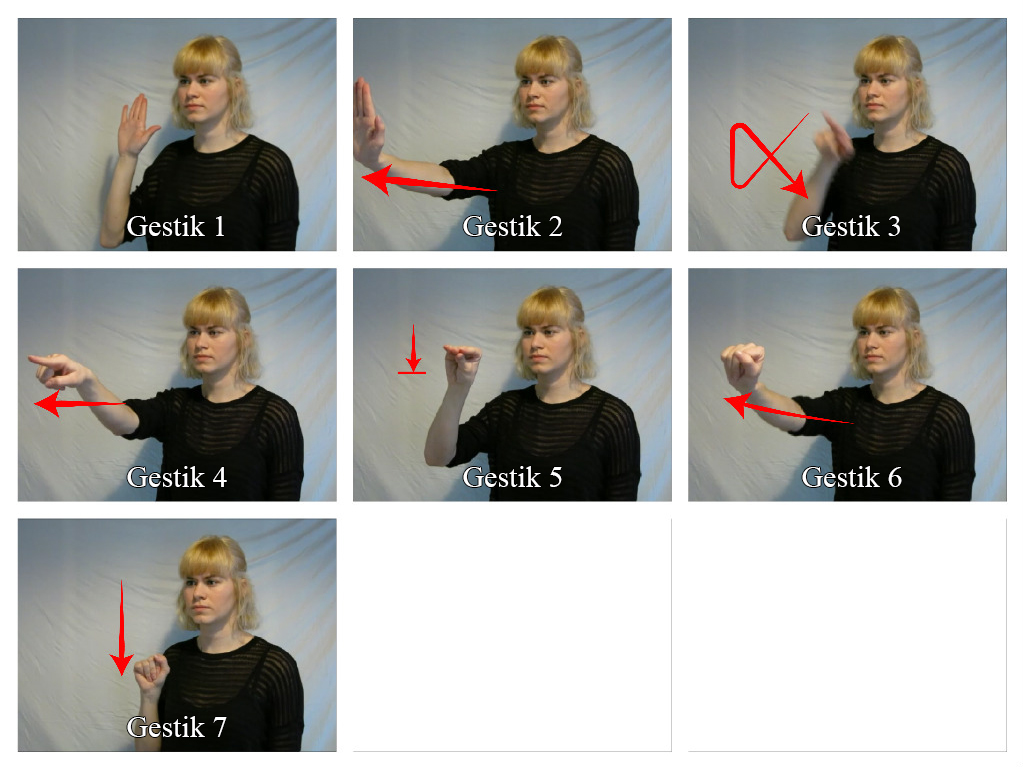
\includegraphics[resolution=300,width=0.70\textwidth, angle=-90]{collage_start_pause_tekst}
%	\caption{Oversigts-billede af alle gestikker, der pauser og starter musikken, fra videoen, inklusiv nummerering og pile, der viser retningen af bevægelsen.}
%	\label{fig:OversigtPauseStart}
%\end{figure}
%\noindent
%
%
%\begin{figure}[H]
%	\centering
%	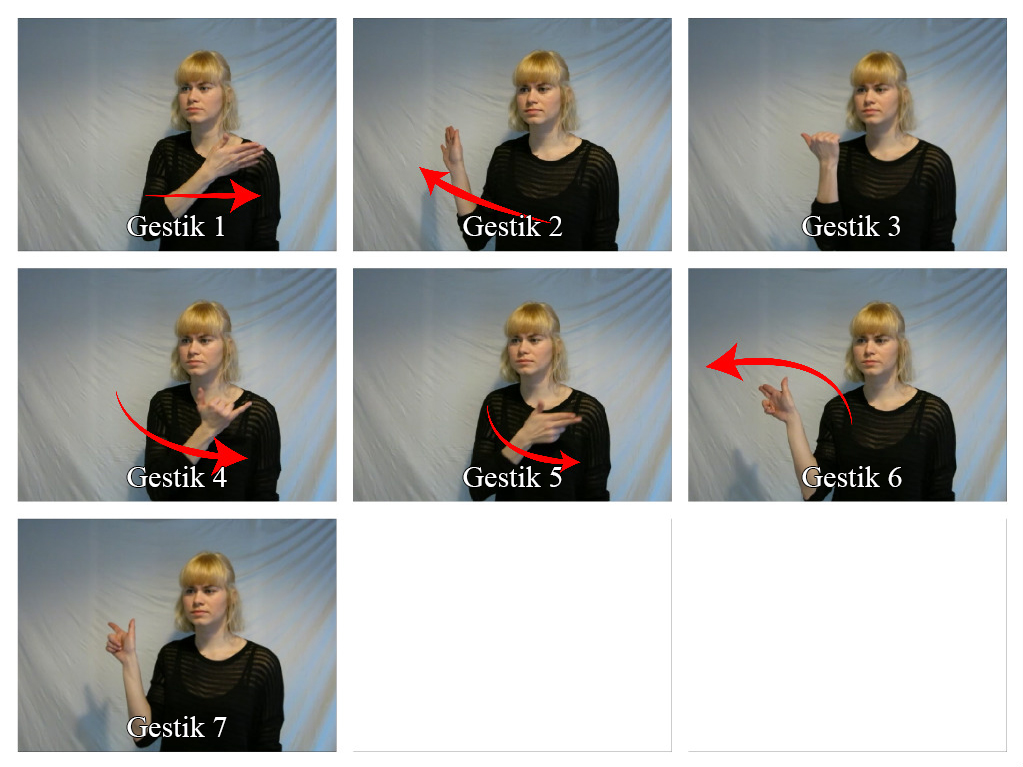
\includegraphics[resolution=300,width=0.70\textwidth, angle=-90]{collage_Skiftsang_tekst}
%	\caption{Oversigts-billede af alle gestikker, der skifter musiknummer, fra videoen, inklusiv nummerering og pile, der viser retningen af bevægelsen. }
%	\label{fig:OversigtSkift}
%\end{figure}
%\noindent
%
%
%\begin{figure}[H]
%	\centering
%	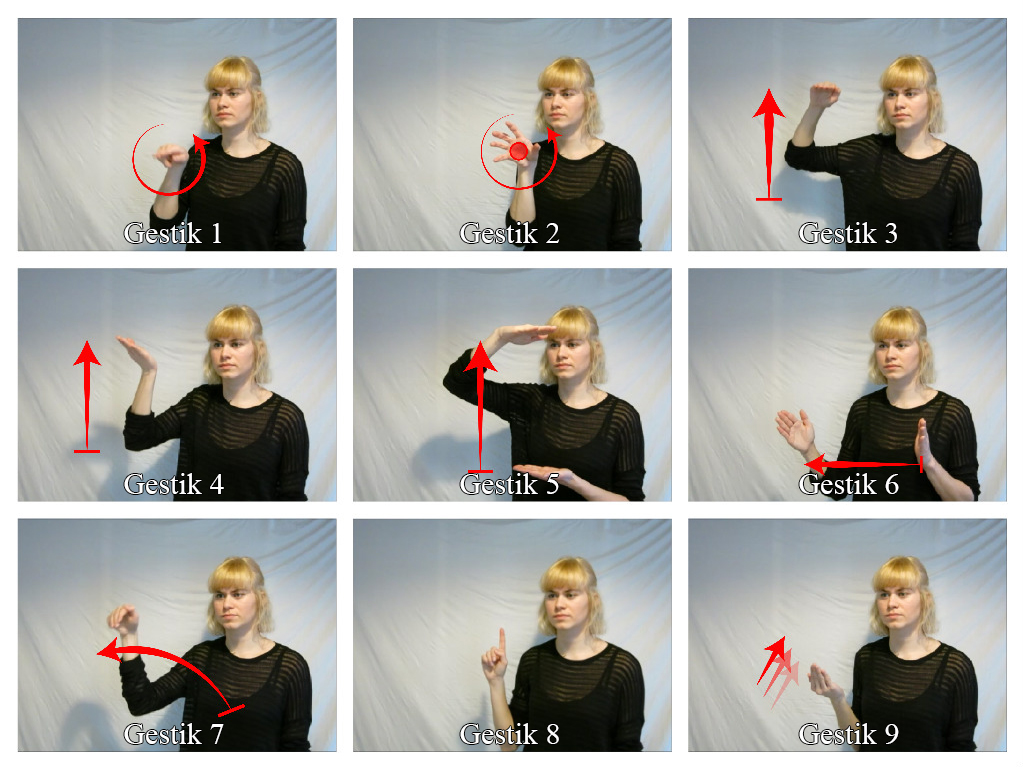
\includegraphics[resolution=300,width=0.70\textwidth, angle=-90]{collage_volumen_tekst}
%	\caption{Oversigt-billede af alle gestikker, der ændrer volumen af musikken, fra videoen, inklusiv nummerering og pile, der viser retningen af bevægelsen.}
%	\label{fig:OversigtVolumen}
%\end{figure}
%\noindent
%

Da forslag til gestikker, der kan tilknyttes de forskellige funktioner, nu er udvalgt og demonstreret, vil det følgende omhandle de forskellige aspekter af den test, der skal være med til at bestemme hvilke gestikker der skal knyttes til de specifikke funktioner.